\section{Lezione del 28/02/2018}

\subsection{Problem Solving}
\begin{enumerate}
	\item Formalizzazione del problema;
	\item Sviluppo dell'\textbf{algoritmo} (focus del corso);
	\item Implementazione in un programma (codice).
\end{enumerate}

\paragraph{Algoritmo} Sequenza di passi elementari che risolve il problema.\par

\begin{center}
	Input $\rightarrow$ \textbf{Algoritmo} $\rightarrow$ Output
\end{center}

\begin{quote} 
	\textit{Dato un problema, ci sono tanti algoritmi per risolverlo.}
\end{quote}

\paragraph{e.g.} Ordinamento dei numeri di una \texttt{Rubrica}.
L'idea è quella di trovare tutte le permutazioni di ogni numero.\par

\begin{center}
	30 numeri: \textit{complessità} $30! \cong 2 \times 10^{32}$ns $\Rightarrow$ \\
	$3^{19}$ anni (con \textit{ns} = nanosecondi)
\end{center}

\paragraph{std::vector} È un esempio nel \texttt{C++} delle ragioni per cui si studia questa materia. Nella documentazione della \texttt{STL}, sono riportati i seguenti:

\begin{itemize}
	\item \texttt{Random access}: complessità O(1);
	\item \texttt{Insert}: complessità O(1) ammortizzato.
\end{itemize}

Il \texttt{random access} è l'accesso a un elemento casuale del \texttt{vector}. O(1) implica che l'accesso avviene in tempo costante (pari a 1). \\
Per \texttt{insert} si intende l'inserimento di un nuovo elemento in coda. Avviene in tempo O(1) ammortizzato: questo perchè ogni N inserimenti, è necessario un resize del vector e una copia di tutti gli elementi nel nuovo vettore.

\subsection{Cosa analizzeremo nel corso}

\begin{itemize}
	\item Tempo di esecuzione;
	\item Spazio (memoria);
	\medskip
	\item[$\circ$] Correttezza;
	\item[$\circ$] Manutenibilità.
\end{itemize}

\subsubsection{Approfondimento sul tempo di esecuzione T(n)}

\begin{figure}[htb]
	\centering
	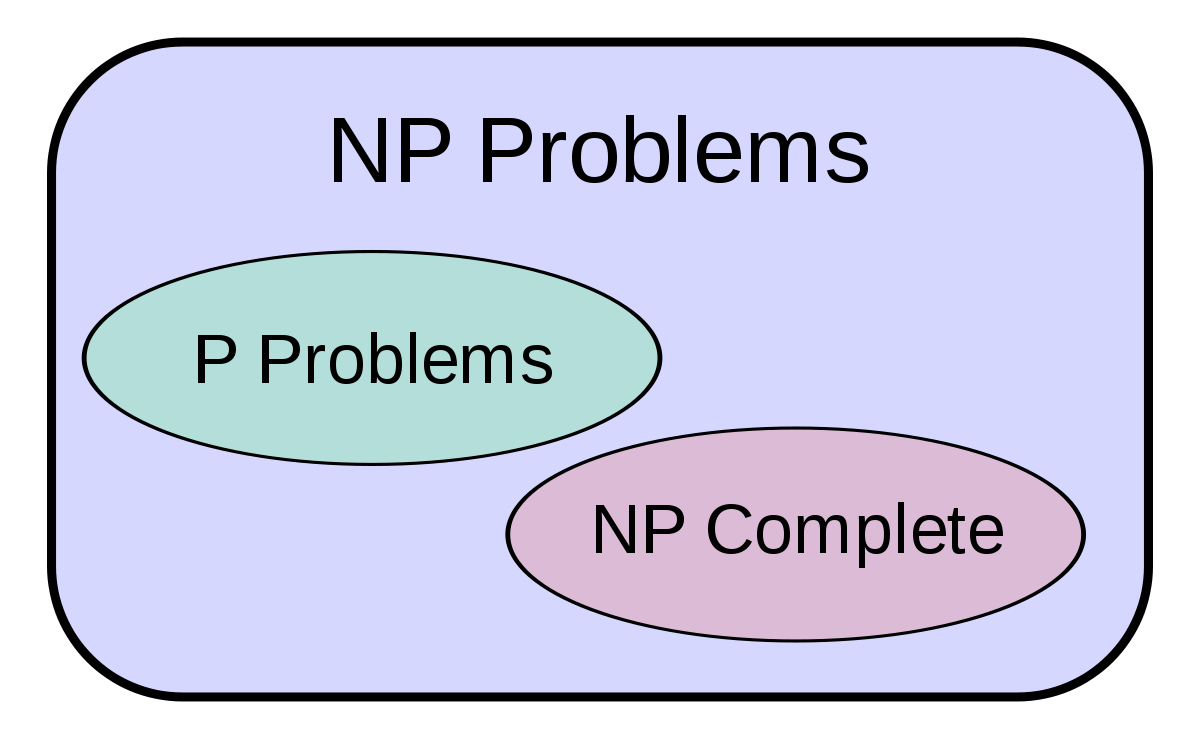
\includegraphics[height=6cm]{img/algorithm_complexity.png}
	\caption{Complessità T(n).}	
\end{figure}

\begin{itemize}
	\item \textit{P Problems}: complessità polinomiale. L'algoritmo è trattabile
	\item \textit{NP Complete}: problemi NP completi. \textbf{e.g}: Applicazione sugli algoritmi di sicurezzza. Si basano sull'assunzione che per essere risolti debbano essere considerate tutte le soluzioni possibili.
	\item \textit{NP Problems}: problemi con complessità  (ad esempio) esponenziale/fattoriale. Assolutamente non trattabili.
\end{itemize}
	
\subsection{Problema dell'ordinamento (sorting)}
\texttt{Input}: sequenza di numeri 
\begin{center}
	$a_0 a_1 \dots a_n$;\par
\end{center}
\texttt{Output}: permutazione
\begin{center}
	$a'_0 a'_1 \dots a'_n$
\end{center}
tale che 
\begin{center}
	$a'_0 \leq a'_1 \leq \dots \leq a'_n$
\end{center}

Vedremo due algoritmi:
\begin{itemize}[noitemsep]
	\item \texttt{Insertion Sort};
	\item \texttt{Merge Sort}.
\end{itemize}

\subsection{Insertion Sort}
È l'algoritmo di sorting che viene fatto naturalmente ad esempio quando si vogliono ordinare le carte nella propria mano in una partita a scala 40: si prende ogni carta a partire da sinistra, e la si posiziona in ordine crescente.\par
\paragraph{Astrazione} Prendiamo ad esempio il seguente array:

\begin{center}
	\begin{tabular}{|l|l|l|l|l|}
		\hline
		5 & 2 & 8 & 4 & 7 \\
		\hline
	\end{tabular}
\end{center}
	
Partiamo dal primo elemento: 5. È già ordinato con se stesso, quindi procediamo con il secondo elemento.\par
Il numero 2 lo confronto con l'elemento alla sua destra: \par
$2 \geq 5$?  No, quindi lo inverto con l'elemento alla sua sinistra, come segue

\begin{center}
	\begin{tabular}{|l|l|l|l|l|}
		\hline
		2 & 5 & 8 & 4 & 7 \\
		\hline
	\end{tabular}
	\hspace{1cm} Key: 
	\begin{tabular}{|l|}
		\hline
		8 \\
		\hline
	\end{tabular}
\end{center}

La key analizzata è 8. \par
$8 \geq 5$? Sì, quindi è ordinato in modo corretto.

\begin{center}
	\begin{tabular}{|l|l|l|l|l|}
		\hline
		2 & 5 & 8 & 4 & 7 \\
		\hline
	\end{tabular}
	\hspace{1cm} Key: 
	\begin{tabular}{|l|}
		\hline
		4 \\
		\hline
	\end{tabular}
\end{center}

La key analizzata è 4.\par
$4 \geq 8$? No, quindi lo sposto a sinistra invertendolo con 8.\par 
$4 \geq 5$? No, lo sposto a sinistra invertendolo con 5.\par
$4 \geq 2$? Sì, quindi è nella posizione corretta.

\begin{center}
	\begin{tabular}{|l|l|l|l|l|}
		\hline
		2 & 4 & 5 & 8 & 7 \\
		\hline
	\end{tabular}
	\hspace{1cm} Key: 
	\begin{tabular}{|l|}
		\hline
		7 \\
		\hline
	\end{tabular}
\end{center}

Key analizzata 7. \par
$7 \geq 8$? No, lo sposto a sinistra invertendolo con 8.\par
$7 \geq 5$? Sì, è nella posizione corretta.\par
\smallskip
Ottengo l'array ordinato:

\begin{center}
	\begin{tabular}{|l|l|l|l|l|}
		\hline
		2 & 4 & 5 & 7 & 8 \\
		\hline
	\end{tabular}
\end{center}

\newpage

\paragraph{Algorimo} Passiamo ora all'implementazione dell'algoritmo, con uno pseudocodice similare a \texttt{Python}\footnote{\textbf{ATTENZIONE}: verranno usati array con indici
che partono da 1.}\par

\bigskip

\texttt{Input}: $A[1, \dots ,n]$, $A.length$.

\begin{center}
	È noto che: 
	$A[i] \leq key < A[i+1]$
\end{center}

\paragraph{Pseudocodice} Segue lo pseudocodice dell'\texttt{Insertion Sort}.

\begin{lstlisting}
  n = A.length
  for j = 2 to n  #il primo elemento e' gia' ordinato
    key = A[j]    #[1...j-1] ordinato
    i = j-1
    while (i > 0) and (A[i] > key)
      A[i+1] = A[i]
      i = i-1
    A[i+1 = key]
\end{lstlisting}

\vspace{0.5cm}

Se il \texttt{while} termina, ci sono due casi: 
\begin{itemize}
	\item[$\circ$] \texttt{i = 0}: tutti gli elementi prima di \texttt{j} 
	sono maggiori di \texttt{key}; \texttt{key} va al primo posto (1);
	\item[$\circ$] \texttt{(i > 0) and (A[i] $\leq$ key)}: \texttt{A[i+1] = key}.
\end{itemize}

\subsubsection{Invarianti e correttezza}

\paragraph{for} \texttt{A[1\dots j-1]} è ordinato e contiene gli 
elementi in \texttt{(1,j-1)} iniziali.

\paragraph{while} \texttt{A[1\dots i]A[i+2\dots j]} ordinato e 
\texttt{A[i+2\dots j] > key}. \par
\vspace{0.5cm}
In uscita abbiamo: 
\begin{itemize}[noitemsep]
	\item[$\circ$] \texttt{j = n+1}; \par
	\item[$\circ$] \texttt{A[1\dots n]} ordinato, come da invariante: 
	vale \texttt{A[1\dots j-1]}	ordinato, e \texttt{j} vale \texttt{n+1}.
\end{itemize}